\documentclass[nolayout]{article}

\usepackage[utf8]{inputenc}
\usepackage[english]{babel}
\usepackage{amsmath,amsthm}
\usepackage{geometry}
\usepackage{tikz}
\usetikzlibrary{fit,positioning}
\usepackage[textwidth=4cm,textsize=footnotesize]{todonotes}
\usepackage{fancyhdr}
\pagestyle{fancy}
\usepackage{amssymb,color,bbm,xargs}
\usepackage{graphicx}
\usepackage[active]{srcltx}
\usepackage{ifthen}
\usepackage{enumerate}
\usepackage{dsfont}
\usepackage{subcaption}

\newtheorem{lemma}{Lemma}
\newtheorem{proposition}{Proposition}
\newtheorem{theorem}{Theorem}
\newtheorem{corollary}{Corollary}

\definecolor{lavander}{cmyk}{0,0.48,0,0}
\definecolor{violet}{cmyk}{0.79,0.88,0,0}
\definecolor{burntorange}{cmyk}{0,0.52,1,0}
\definecolor{burntgreen}{cmyk}{0.62,0.44,0.47,0}
\definecolor{burntblue}{cmyk}{0.86,0.30,0.18,0}
\definecolor{palegreen}{cmyk}{0.86,0.30,0.96,0}


\def\sup{\mathrm{sup}}
\def\param{\theta}
\def\paramset{\Theta}
\def\1{\mathds{1}}
\def\rset{\mathbb{R}}
\def\rmd{\mathrm{d}}
\def\eqsp{\,}
\def\Pstar{\mathbb{P}_{\pi_{\star}}}
\def\bayes{\pi_{\star}}
\def\kernel{\mathsf{M}}
\newcommand{\limit}[1]{\underset{#1\to \infty}{\longrightarrow}}
\newcommand{\E}{\mathbb{E}}
\newcommand{\kullback}{\mathsf{L}}
\newcommand{\link}{\leftrightarrow}


\newcommand{\pa}[1]{\left(#1\right)}
\newcommand{\cro}[1]{\left[#1\right]}
\newcommand{\set}[1]{\left\{#1\right\}}
\newcommand{\PE}[1]{\left\lfloor#1\right\rfloor}

\newcommand{\loss}[1]{\ell\pa{#1}}
\newcommand{\Lo}[2]{\ell^{#1}\pa{#2}}

\newcommand{\bN}{\mathbb{N}}
\newcommand{\bP}{\mathbb{P}}
\newcommand{\bR}{\mathbb{R}}
\newcommand{\bZ}{\mathbb{Z}}

\newcommand{\cA}{\mathcal{A}}
\newcommand{\cD}{\mathcal{D}}
\newcommand{\cE}{\mathcal{E}}
\newcommand{\cO}{\mathcal{O}}
\newcommand{\cS}{\mathcal{S}}
\newcommand{\cV}{\mathcal{V}}
\newcommand{\cX}{\mathcal{X}}

\newcommand{\ordermax}[2]{{\mathsf{q}}^{#1}_{#2}}
\newcommand{\remainder}[2]{{\mathsf{r}}^{#1}_{#2}}

\newcommand{\condlik}{k}
\newcommand{\card}{\mathrm{card}}

\newcommand{\MLE}{\widehat{\pi}}

\newcounter{hypH}
\newenvironment{hypH}{\refstepcounter{hypH}\begin{itemize}
\item[{\bf H\arabic{hypH}}]}{\end{itemize}}
\begin{document}

\title{Maximum likelihood estimation for the Bradley-Terry model in random environment}
\date{}

\author{}

\lhead{}
\rhead{MLE for the Bradley-Terry model in random environment}

\maketitle

\begin{abstract}

\end{abstract}

\section*{Bradley-Terry model in the case $n=2$}
Let $N$ be the number of players and $(v_i)_{1\le i\le N}$ be the scores associated with each player. It is assumed that the $(v_i)_{1\le i\le N}$ are i.i.d. and that the distribution of $v_1$ has probability density function $\pi_{\param}$ on $C_{\param}\subset \rset_+^{\star}$ with respect to a reference measure $\mu$. Conditional on $(v_i)_{1 \le i \le N}$, the observations $(X_{1,2},X_{1,3}, X_{2k-2,2k}, X_{2k-1,2k+1})_{2\le k \le (N-1)/2}$ are independent and, for each $1\le \ell\le N-2$, the conditional distribution of $X_{\ell,\ell+2}$ given $(v_i)_{1\le i\le N}$ has probability density function:
\begin{equation}
\label{eq:defG}
x\mapsto G (x;v_{\ell},v_{\ell+2}) = \frac{v_{\ell}^x\,v_{\ell+2}^{1-x}}{v_{\ell} + v_{\ell+2}}
\end{equation}
with respect to the counting measure. The conditional distribution of $X_{1,2}$ given $(v_i)_{1\le i\le N}$ has probability density function $x\mapsto G (x;v_{1},v_{2})$ with respect to the counting measure.
The graphical model associated with Bradley-Terry model in the case $n=2$ is displayed in Figure~\ref{fig:bt}.
\begin{figure}[h!]
\centering
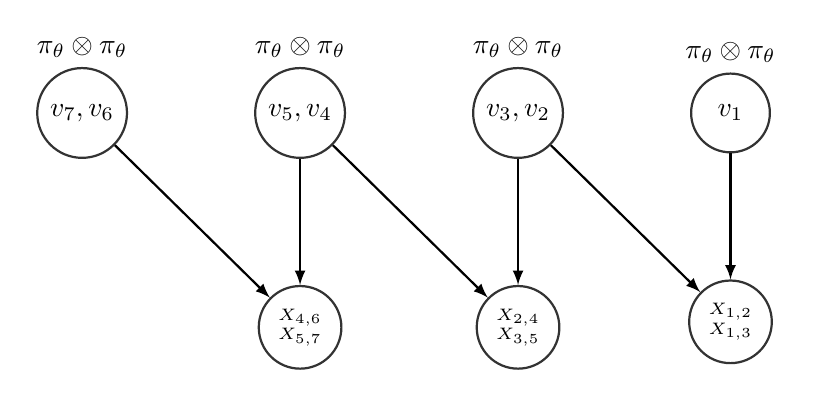
\begin{tikzpicture}
\tikzstyle{main}=[circle, minimum size = 10mm, thick, draw =black!80, node distance = 16mm]
\tikzstyle{connect}=[-latex, thick]
\tikzstyle{box}=[rectangle, draw=black!100]
  \node[main,label=above:$\pi_{\param}\otimes\pi_{\param}$] (v4) {$v_{7}, v_{6}$};
  \node[main,label=above:$\pi_{\param}\otimes\pi_{\param}$] (v3) [right=of v4] {$v_5, v_4$};
  \node[main,label=above:$\pi_{\param}\otimes\pi_{\param}$] (v2) [right=of v3] {$v_3, v_2$};
  \node[main,label=above:$\pi_{\param}\otimes\pi_{\param}$] (v1) [right=of v2] {$v_1$};
  \node[main] (X3) [below=of v3] {{\small $\substack{X_{4,6}\\ X_{5,7}}$}};
  \node[main] (X2) [below=of v2] {{\small $\substack{X_{2,4}\\ X_{3,5}}$}};
  \node[main] (X1) [below=of v1] {{\small $\substack{X_{1,2}\\ X_{1,3}}$}};
  \path (v1) edge [connect] (X1)
           (v2) edge [connect] (X1)
           (v2) edge [connect] (X2)
	   (v3) edge [connect] (X2)
           (v3) edge [connect] (X3)
           (v4) edge [connect] (X3);
\end{tikzpicture}
\caption{Bradley-Terry graphical model in the case $n=2$ and $N=7$.}
\label{fig:bt}
\end{figure}

Consider the following assumptions on the model.

\begin{hypH}
\label{assum:strongmix}
There exist $0<\sigma_-<\sigma_+<\infty$ such that for all $\param\in\param$ and all $v\in C_{\param}$, $\sigma_-\le \pi_{\param}(v)\le\sigma_+$.
\end{hypH}

\begin{hypH}
\label{assum:compact}
There exist $0<c_-<c_+<\infty$ such that for all $\param\in\param$, $C_{\param} \subset (c_-,c_+)$.
\end{hypH}

Define 
\begin{equation}
\label{eq:def:rho}
\rho = 1- \left(\frac{c_-\sigma_-}{(c_-+c_+)\sigma_+}\right)^2\eqsp.
\end{equation}

Define $\bar C_{\param} = C_{\param}\times C_{\param}$, $\bar v_1 = v_1$, $\bar X_1 = (X_{1,2},X_{1,3})$ and for all $k\ge 2$, $\bar v_k = (v_{2k-2},v_{2k-1})$ and $\bar X_k = (X_{2k-2,2k},X_{2k-1,2k+1})$. Conditional on $(\bar v_i)_{i\ge 1}$, the observations $(\bar X_i)_{i\ge 1}$ are independent and, for each $\ell\ge 1$ the conditional distribution of $\bar X_{\ell}$ given $(\bar v_i)_{i\ge 1}$ has probability density function:
\[
\bar x = (x_1,x_2) \mapsto \bar G (\bar x;\bar v_{\ell+1},\bar v_{\ell}) = G (x_1,v_{2\ell},v_{2\ell+2})G (x_2;v_{2\ell-1},v_{2\ell+1})\eqsp,
\]
where $G$ is defined by \eqref{eq:defG}.
\begin{figure}
\label{fig:bt:extended}
\centering
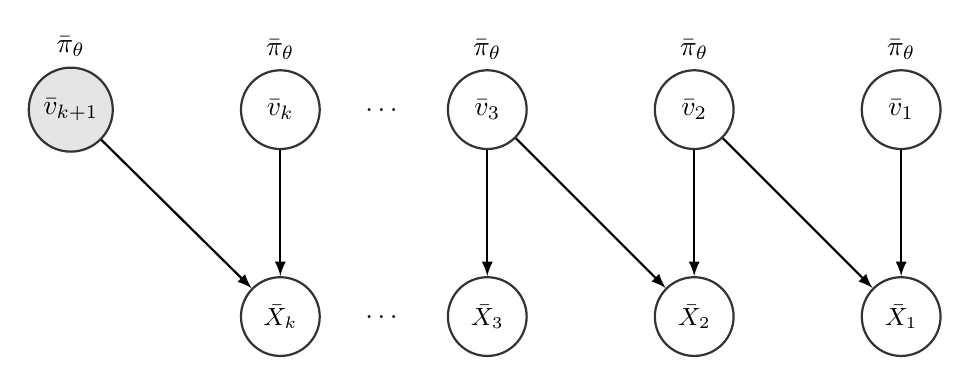
\begin{tikzpicture}
\tikzstyle{main}=[circle, minimum size = 10mm, thick, draw =black!80, node distance = 16mm]
\tikzstyle{connect}=[-latex, thick]
\tikzstyle{box}=[rectangle, draw=black!100]
  \node[main, fill = black!10,label=above:$\bar \pi_{\param}$] (v5){$\bar v_{k+1}$ };
  \node[main,label=above:$\bar \pi_{\param}$] (v4) [right=of v5] {$\bar v_{k}$ };
  \node[main,label=above:$\bar \pi_{\param}$] (v3) [right=of v4] {$\bar v_3$};
  \node[main,label=above:$\bar \pi_{\param}$] (v2) [right=of v3] {$\bar v_2$};
  \node[main,label=above:$\bar \pi_{\param}$] (v1) [right=of v2] {$\bar v_1$};
  \node[main] (X4) [below=of v4] {{\small $\bar X_{k}$}};
  \node[main] (X3) [below=of v3] {{\small $\bar X_{3}$}};
  \node[main] (X2) [below=of v2] {{\small $\bar X_{2}$}};
  \node[main] (X1) [below=of v1] {{\small $\bar X_{1}$}};
  \path (v1) edge [connect] (X1)
           (v2) edge [connect] (X1)
           (v2) edge [connect] (X2)
	   (v3) edge [connect] (X2)
           (v3) edge [connect] (X3)
           (v5) edge [connect] (X4)
           (v4) edge [connect] (X4);
  \path (v4) -- node[auto=false]{\ldots}  (v3);  
  \path (X4) -- node[auto=false]{\ldots} (X3);        
\end{tikzpicture}
\caption{Bradley-Terry graphical model in the case $n=2$ with extended states.}
\end{figure}

\subsection*{Forgetting properties of the Bradley-Terry model}
For all $1\le k < n$ and all probability density function $\lambda$ on $\bar C_{\param}$, denote by $\phi^{n,k}_{\lambda,\param}$ the probability density of the conditional distribution of $\bar v_k$ given $(\bar X_n,\ldots,\bar X_k)$ when the state $\bar v_{n+1}$ has probability density function $\lambda$ on $\bar C_{\param}$. Note that for all $1\le k \le n < m$,
\begin{align*}
\phi^{m,k}_{\lambda,\param}\left(\bar v_{k}\right) &= \frac{\int \lambda(\bar v_{m+1})\prod_{i = m}^k\bar G(\bar X_i; \bar v_{i+1},\bar v_i) \bar \pi_{\param}(\bar v_i)\mu(\rmd \bar v_{m+1:k+1})}{\int \lambda(\bar v_{m+1})\prod_{i = m}^k\bar G(\bar X_i; \bar v_{i+1},\bar v_i) \bar \pi_{\param}(\bar v_i)\mu(\rmd \bar v_{m+1:k})} = \phi^{n,k}_{\eta^{m,n}_{\lambda,\param},\param}\left(\bar v_{k}\right)\eqsp,
\end{align*}
where, $\eta^{m,n}_{\lambda,\param}$ is the probability density function defined on $\bar C_{\param}$ as:
\[
\eta^{m,n}_{\lambda,\param}: \bar v_{n+1} \mapsto \frac{\int \lambda(\bar v_{m+1})\bar G(\bar X_m; \bar v_{m+1},\bar v_m)\prod_{i = m}^{n+2} \bar \pi_{\param}(\bar v_i) \bar G(\bar X_{i-1}; \bar v_{i},\bar v_{i-1}) \mu(\rmd \bar v_{m+1:n+2})}{\int \lambda(\bar v_{m+1})\bar G(\bar X_m; \bar v_{m+1},\bar v_m)\prod_{i = m}^{n+2} \bar \pi_{\param}(\bar v_i) \bar G(\bar X_{i-1}; \bar v_{i},\bar v_{i-1}) \mu(\rmd \bar v_{m+1:n+1})}\eqsp.
\]
For all $n\ge1$, and all $\param\in\param$, the likelihood of the observations is given by:
\[
L^n_{\pi_{\param},\param}\left(\bar X_{1},\ldots,\bar X_{n}\right) = p_{\pi_{\param},\param}\left(\bar X_n\right)\prod_{k=1}^{n-1}p_{\pi_{\param},\param}\left(\bar X_{k}\middle| \bar X_{n},\ldots,\bar X_{k+1}\right)
\] 
and the loglikelihood is written:
\[
\ell^n_{\pi_{\param},\param}\left(\bar X_{1},\ldots,\bar X_{n}\right) = \log L^n_{\pi_{\param},\param}\left(\bar X_{1},\ldots,\bar X_{n}\right) = \log p_{\pi_{\param},\param}\left(\bar X_n\right) + \sum_{k=1}^{n-1}\log p_{\pi_{\param},\param}\left(\bar X_{k}\middle| \bar X_{n},\ldots,\bar X_{k+1}\right)\eqsp.
\]
For all $2\le k\le n <m$,
\begin{equation}
\label{eq:incremental:likelihood}
p_{\pi_{\param},\param}\left(\bar X_{k}\middle| \bar X_{n},\ldots,\bar X_{k+1}\right) = \int_{\bar C_{\param}^2}\phi^{n,k+1}_{\pi_{\param},\param}\left(\bar v_{k+1}\right)\pi_{\param}(\bar v_{k})\bar G(\bar X_{k};\bar v_{k+1},\bar v_{k})\mu(\rmd \bar v_{k:k+1})
\end{equation}
and 
\begin{align*}
p_{\pi_{\param},\param}\left(\bar X_{k}\middle| \bar X_{m},\ldots,\bar X_{k+1}\right) &= \int_{\bar C_{\param}^2}\phi^{m,k+1}_{\pi_{\param},\param}\left(\bar v_{k+1}\right)\pi_{\param}(\bar v_{k})\bar G(\bar X_{k};\bar v_{k+1},\bar v_{k})\mu(\rmd \bar v_{k:k+1})\eqsp,\\
&=\int_{\bar C_{\param}^2}\phi^{n,k+1}_{\eta^{m,n}_{\pi_{\param},\param},\param}\left(\bar v_{k+1}\right)\pi_{\param}(\bar v_{k})\bar G(\bar X_{k};\bar v_{k+1},\bar v_{k})\mu(\rmd \bar v_{k:k+1})\eqsp.
\end{align*}
\begin{lemma}
Assume that H\ref{assum:strongmix} and H\ref{assum:compact} hold. Then, for all $1\le k \le n < m$, $\Pstar$-a.s.,
\[
\sup_{\theta\in\Theta}\left|\log p_{\pi_{\param},\param}\left(\bar X_{k}\middle| \bar X_{n},\ldots,\bar X_{k+1}\right) - \log p_{\pi_{\param},\param}\left(\bar X_{k}\middle| \bar X_{m},\ldots,\bar X_{k+1}\right)\right| \le \left(1+\frac{c_+}{c_-}\right)^2\rho^{n-k}\eqsp,
\]
where $\rho$ is defined by \eqref{eq:def:rho}.
In addition,
\[
\sup_{\theta\in\Theta;\;n\ge k}\left|\log p_{\pi_{\param},\param}\left(\bar X_{k}\middle| \bar X_{n},\ldots,\bar X_{k+1}\right)\right|\le 2\log\left(1+\frac{c_+}{c_-}\right)\eqsp. 
\]
\end{lemma}
\begin{proof}
To prove the first inequality, note that
\begin{multline}
\left|p_{\pi_{\param},\param}\left(\bar X_{k}\middle| \bar X_{n},\ldots,\bar X_{k+1}\right) - p_{\pi_{\param},\param}\left(\bar X_{k}\middle| \bar X_{m},\ldots,\bar X_{k+1}\right)\right|\\
= \left|\left(\phi^{n,k+1}_{\eta^{m,n}_{\pi_{\param},\param},\param} - \phi^{n,k+1}_{\pi_{\param},\param}\right)\left[\int_{\bar C_{\param}}\pi_{\param}(\bar v_{k})\bar G(\bar X_{k};\cdot,\bar v_{k})\mu(\rmd \bar v_{k})\right]\right|\eqsp.\label{eq:diff:likelihood}
\end{multline}
Conditional on $(\bar X_n,\ldots,\bar X_{k+1})$, $(\bar v_{n+1},\ldots,\bar v_{k+1})$ is a Markov chain with kernel:
\begin{align*}
p_{\param}\left(\bar v_{p}\middle | \bar v_{n+1},\ldots, \bar v_{p+1},\bar X_n,\ldots,\bar X_{k+1}\right) &=  p_{\param}\left(\bar v_{p}\middle |\bar v_{p+1},\bar X_p,\ldots,\bar X_{k+1}\right)\eqsp,\\
&\propto \bar\pi_{\param}(\bar v_{p+1}) \bar G(\bar X_{p};\bar v_{p+1},\bar v_{p})p_{\param}\left(\bar X_{p-1},\ldots,\bar X_{k}\middle|\bar v_p\right)\eqsp.
\end{align*}
Therefore, by H\ref{assum:strongmix} and H\ref{assum:compact}, for all measurable set $A\subset \bar C_{\param}$,
\[
\mathbb{P}_{\param}\left(\bar v_{p}\in A\middle | \bar v_{n+1},\ldots, \bar v_{p+1},\bar X_n,\ldots,\bar X_{k+1}\right) \ge \left(\frac{c_-\sigma_-}{(c_-+c_+)\sigma_+}\right)^2 \mu^p_{\param}\left(\bar X_{p-1},\ldots,\bar X_{k},A\right)\eqsp,
\]
where the measure $\mu^p_{\param}\left(\bar X_{p-1},\ldots,\bar X_{k},\cdot\right)$ is given by
\[
\mu^p_{\param}\left(\bar X_{p-1},\ldots,\bar X_{k},A\right) = \frac{\int_{\bar C_{\param}} \1_{A}(\bar v_p)p_{\param}\left(\bar X_{p-1},\ldots,\bar X_{k}\middle|\bar v_p\right)\mu(\rmd \bar v_p)}{\int_{\bar C_{\param}} p_{\param}\left(\bar X_{p-1},\ldots,\bar X_{k}\middle|\bar v_p\right) \mu(\rmd \bar v_p)}\eqsp.
\]
By \eqref{eq:diff:likelihood}, as the function $G$ is upper bounded by $1$,
\begin{align*}
\left|p_{\pi_{\param},\param}\left(\bar X_{k}\middle| \bar X_{n},\ldots,\bar X_{k+1}\right) - p_{\pi_{\param},\param}\left(\bar X_{k}\middle| \bar X_{m},\ldots,\bar X_{k+1}\right)\right| &\le \rho^{n-k} \sup_{\bar v} \int_{\bar C_{\param}}\pi_{\param}(\bar v_{k})\bar G(\bar X_{k};\bar v,\bar v_{k})\mu(\rmd \bar v_{k})\eqsp,\\
&\le \rho^{n-k}\eqsp.
\end{align*}
In addition, by \eqref{eq:incremental:likelihood}, 
\[
p_{\pi_{\param},\param}\left(\bar X_{k}\middle| \bar X_{n},\ldots,\bar X_{k+1}\right)\wedge p_{\pi_{\param},\param}\left(\bar X_{k}\middle| \bar X_{m},\ldots,\bar X_{k+1}\right)\ge \left(\frac{c_-}{c_-+c_+}\right)^2\eqsp.
\]
As for all $x,y>0$, $|\log x - \log y| \le |x-y|/x\wedge y$,
\[
\left|\log p_{\pi_{\param},\param}\left(\bar X_{k}\middle| \bar X_{n},\ldots,\bar X_{k+1}\right) - \log p_{\pi_{\param},\param}\left(\bar X_{k}\middle| \bar X_{m},\ldots,\bar X_{k+1}\right)\right| \le \left(1+\frac{c_+}{c_-}\right)^2\rho^{n-k}\eqsp.
\]
The second inequality follows from \eqref{eq:incremental:likelihood} and the fact that the function $G$ defined by \eqref{eq:defG} is upper bounded by $1$ and lower bounded by $c-/(c_-+c_+)$.
\end{proof}
\end{document}